\documentclass[tikz,border=10pt]{standalone}
\usepackage{ctex} % 支持中文（如有需要）
\usetikzlibrary{calc}

\begin{document}

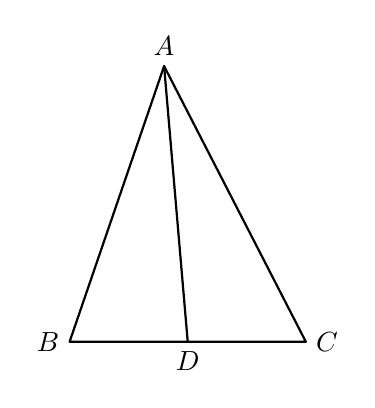
\begin{tikzpicture}[line join=round, line cap=round, >=stealth, thick]
    % 1. 定义顶点坐标 (根据图像比例估算)
    % A为顶点，B, C为底边端点，D为BC上的一点
    \coordinate (A) at (1.2, 3.5);
    \coordinate (B) at (0, 0);
    \coordinate (C) at (3, 0);
    \coordinate (D) at (1.5, 0); % D点位于BC之间

    % 2. 绘制三角形主体
    \draw (A) -- (B) -- (C) -- cycle;

    % 3. 绘制内部线段 AD
    \draw (A) -- (D);

    % 4. 标注顶点标签
    % 使用 anchor 确保标签位置与图片一致：A在上方，B在左侧，C在右侧，D在下方
    \node[above] at (A) {$A$};
    \node[left]  at (B) {$B$};
    \node[right] at (C) {$C$};
    \node[below] at (D) {$D$};

    % (可选) 如果需要标注角度或垂直符号，可以在此处添加
    % 如需标注D点的小圆点（视原图清晰度而定，通常学术图中不加，此处略去）

\end{tikzpicture}

\end{document}